\section{Results}
\label{Results}

% \subsection{Defect Density Prediction}
The Figg. \ref{fig:abn.vs.n.comm} and \ref{fig:cc.vs.n.comm} show the distributions of the average bugs number 
(ABN, Fig. \ref{fig:abn.vs.n.comm}) 
and clustering coefficient (CC, Fig. \ref{fig:cc.vs.n.comm}) with respect to the number of communities (NOC) 
for all the sub-projects of all the releases. 
Whereas the scatterplots for the relationship between NOC 
and other metrics are sparse, the reported scatterplots show that 
there is a power-law-like relationship between the maximum values of the mentioned metrics. 
This led us to hypothesize that there is a linear relationship between the maximum values of CC and the ABN. 
If this was the case, then the CC could be used to predict the maximum ABN s 
in a future release, given the cumulated data from the past.
In Tab. \ref{tab:log-log-cc-NB} 
the power law exponents, the correlation coefficient $r$, the $\chi^2$
and the degrees of freedom (\textit{dof})for the best fitting in log-log scale are reported. 
The latter refer to  the relationship between CC and NOC for different ``cumulated''
releases.
As can been seen by looking at Tab. \ref{tab:log-log-cc}, power laws parameters do not change significantly 
from one cumulated release to another. This seems to suggest that there is a stable behaviour during 
software evolution, when the fitting with a power law becomes more accurate and tends to a fixed value 
as new releases are added in the cumulated dataset.
Same behaviour applies for the relationship between maximum ABN and NOC, as shown in Tab.~\ref{tab:log-log-max-abn-vs-noc}. 

The scatterplot shown on Fig. \ref{cumulated_bug_cc} shows the relationship between the maximum defect 
density versus the maximum clustering coefficient, 
for all the cumulated releases, along with the fitting straight line.
The plot shows a stable behaviour during the evolution the Eclipse project, so it can be used to make predictions about 
the quality of future releases in relation with their topology.
Starting with a dataset of $N$ releases, we investigated if the best fitting curve for the cumulated $N -1$ releases 
could be also a good fit for the $Nth$ releases.

As a measure of prevision accuracy, we adopted a $\chi^2$ test.
In Table 4 we can see the results of the fitting for the relationship between CC and ABN where we can see that 
linear correlation is not high. Nonetheless, $\chi^2$ returns an high significance level.
Table 2 % \ref{prevision_test} 
reports the results of the analysis on the prediction quality. 
We computed the ratio between $\chi^2$ and the degree of freedom. 
% The reported $\chi^2$ values are close to 1, meaning that for the given degrees of freedom the fits are good.
As it can be seen from the values reported on Table \ref{prevision_test}, $\chi^2$ values are close to 1, 
meaning that for the given degrees of freedom the fits are good.


  \begin{minipage}{\textwidth}
  \begin{minipage}{0.3 \textwidth}
    \centering
%     \rule{6.4cm}{3.6cm}
    \vspace{10pt} \includegraphics[width=\textwidth]{figure/EC_BUG_power_law-eps-converted-to.pdf}
    \captionof{figure}{Average Bug Number vs. Number of Communities}
    \label{fig:abn.vs.n.comm}
  \end{minipage}
  \hfill
        \begin{minipage}{0.3 \textwidth}
%           \begin{figure}[H]
              \vspace{0pt} \includegraphics[width=\textwidth]{figure/EC_CC_power_law-eps-converted-to.pdf}
              \captionof{figure}{Clustering Coefficient vs. Number of Communities}
              \label{fig:cc.vs.n.comm}
%           \end{figure}
      \end{minipage}
  \begin{minipage}{0.30\textwidth}
 \vspace{20pt}
    \centering
   
    \resizebox{\columnwidth}{!}{
      \begin{tabular}{|c|c|c|c|c|c|}
	\hline
	\textbf{Eclipse} & max ADD & max CC \\ 	\hline
		     dof & 13 & 13 \\
		    $\chi^2$ / dof & 0.361 & 1.005 \\ \hline
      \end{tabular}
	  }
	  \label{prevision_test}
      \captionof{table}{Values of the $\chi^2$ coefficient and of the reduced degrees of freedom (\textit{dof})
for the fitting of the points from the last release with the line given by the previous releases.
The values refers to the maximum average defect density(max ADD) and to the maximum clustering coefficient (max CC).}
    \end{minipage}
  \end{minipage}
  \vspace{0.01\linewidth}

\begin{table}[htbp]
\begin{center}
% For LaTeX tables use

\begin{tabular}{|c|c|c|c|c|}
\hline
\textbf{Eclipse} &2.1 - 3-0 & 2.1 - 3.1 & 2.1 - 3.2 & 2.1 - 3.3 \\
\hline
$r$ & 0.565  & 0.576 &  0.677 &  0.687\\ 

$\chi^2$ & 0.633& 0.651  & 0.523 & 0.547  \\

$dof$ & 16 & 17 & 20 & 21\\ 
\hline
\end{tabular}

\label{tab:log-log-cc}
\caption{Data regarding maximum Clustering Coefficient vs Number of communities for Eclipse: exponent $\alpha$, 
correlation coefficient ($r$), value of Chi Squared ($\chi^2$ ) and number of degrees of freedom ($dof$).}
% \caption{Data regarding maximum Clustering Coefficient vs Number of communities for NetBeans: exponent $\alpha$, 
% correlation coefficient ($r$), value of Chi Squared ($\chi^2$ ) and number of degrees of freedom ($dof$).}
\end{center}
     % Give a unique label
\end{table}

  \begin{minipage}{\textwidth}
  \begin{minipage}{0.65\textwidth}
%     \centering
    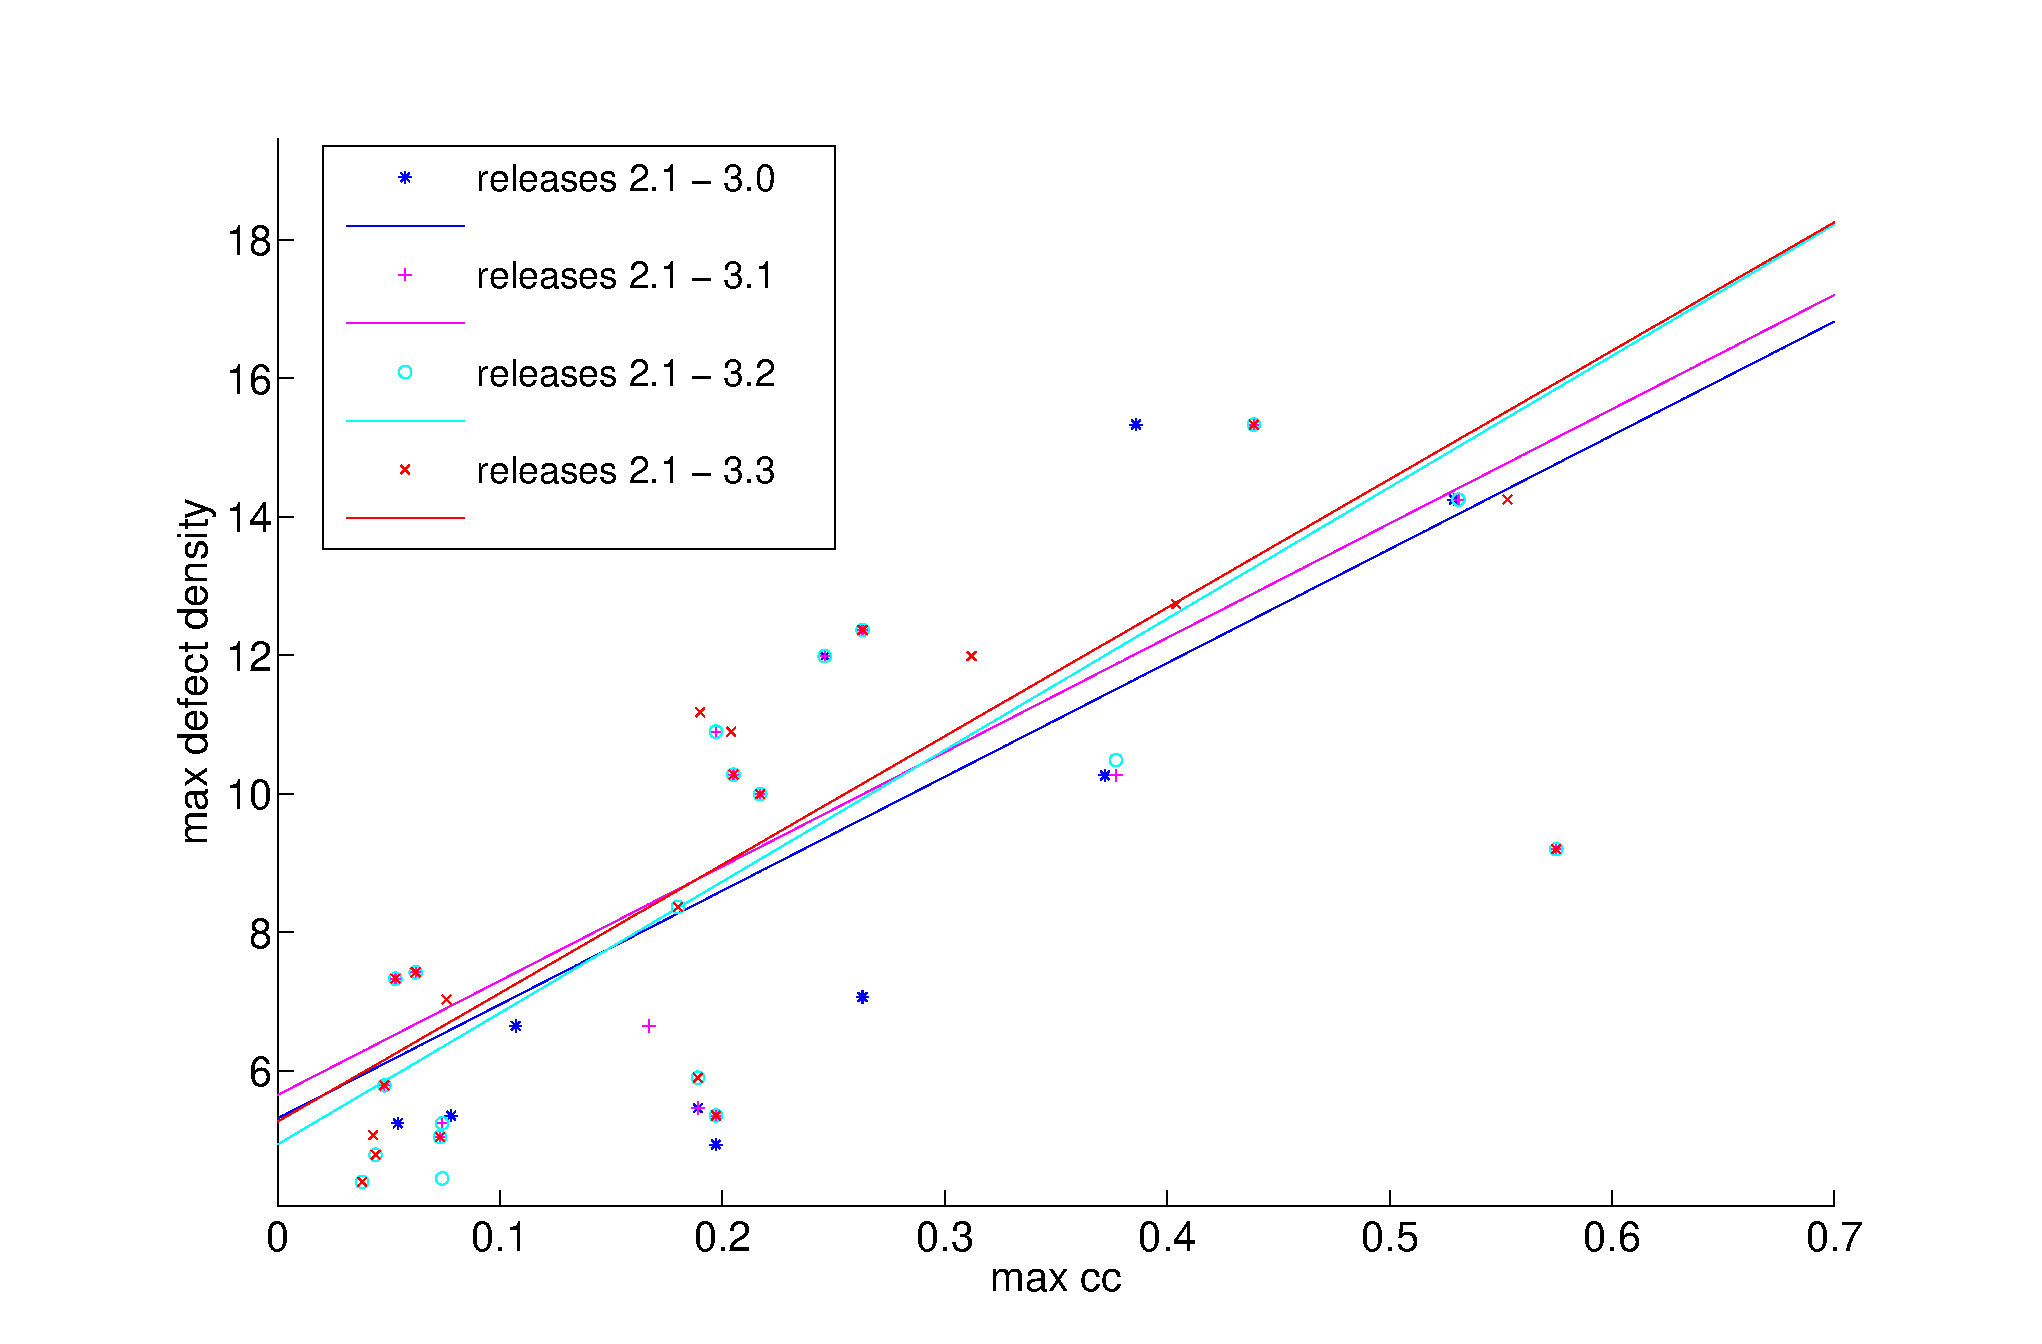
\includegraphics[width=0.9 \textwidth]{figure/nuovefig/cumulated_bug_cc_EC.eps}
    \label{cumulated_bug_cc}
    \captionof{figure}{Cumulated plots and fitting lines for the maximum defect density vs maximum clustering coefficient.}
  \end{minipage}
%   \hfill
  \begin{minipage}{0.30\textwidth}
  \vspace{5pt}
    \centering
    \resizebox{\columnwidth}{!}{
      \begin{tabular}{|l|c|c|c|}
      \hline
      \textbf{Releases} & $r$ & $\chi^2$ & $dof$  \\\hline
      2.1 - 3-0 & 0.565 & 0.633 & 16  \\\hline 
      2.1 - 3.1 & 0.576 & 0.651  & 17  \\\hline 
      2.1 - 3.2 & 0.677 & 0.523 & 20 \\ 
      2.1 - 3.3 & 0.687 & 0.547 & 21 \\\hline
      \end{tabular}
      }
      \captionof{table}{NetBeans: fit data for the maximum defect density vs maximum clustering coefficient: correlation coefficient ($r$), 
      normalized Chi squared ($\chi^2$ ), and number of degrees of freedom ($dof$).}
\label{tab:max_abn-vs-maxcc}       % Give a unique label
    \end{minipage}
  \end{minipage}
